\documentclass[a6paper, parskip=half, DIV=14, 10pt]{scrartcl}
\usepackage{fontspec}
\usepackage[dvipsnames]{xcolor}
\usepackage{tikz}

\usepackage{unicode-math}
\setmathfont{texgyreschola-math.otf}[math-style=TeX]

\usepackage{booktabs}
\usepackage{multicol}
\setlength\columnsep{3em}
\usepackage{enumitem}
\usepackage{caption}
\usepackage{scrlayer-scrpage} % Manage headers and footers in Koma-Script document classes
\setlength{\footskip}{1cm}

\usepackage[type={CC}, version={4.0}, modifier={by}]{doclicense} % Add text and icons for creative commons license
\usepackage{array}
\usepackage{afterpage}

%\usepackage{permutations}
\usepackage{contour}
\contournumber{32}
\usepackage[letterspace=0]{microtype}

\usepackage[hidelinks]{hyperref} % Add hyperlinks to the pdf file. This should usually be the last package loaded before \begin{document}

\setmainfont{TeX Gyre Schola}
\makeatletter
\newcommand{\version}[1]{\newcommand{\@version}{#1}}
\makeatother

% Set header
\clearpairofpagestyles
\makeatletter
\cfoot*{\normalshape Version \@version}
\makeatother

% Minimize unwanted hyphenation
\tolerance=1
\emergencystretch=\maxdimen
\hyphenpenalty=10000
\hbadness=10000

\setkomafont{section}{\setmainfont{Tex Gyre Schola}\Large\bfseries}
\setkomafont{subsection}{\setmainfont{Tex Gyre Schola}\large\bfseries}
\setkomafont{subsubsection}{\setmainfont{Tex Gyre Schola}\normalsize\bfseries}
\setkomafont{descriptionlabel}{\setmainfont{Tex Gyre Schola}\normalsize\bfseries}

\RedeclareSectionCommand[
  runin=false,
  afterindent=false,
  beforeskip=0cm,
  afterskip=0ex,
]{section}

\RedeclareSectionCommand[
  runin=false,
  afterindent=false,
  beforeskip=0pt,
  afterskip=0ex,
]{subsection}

\RedeclareSectionCommand[
  runin=false,
  afterindent=false,
  beforeskip=0pt,
  afterskip=0ex,
]{subsubsection}

\colorlet{permred}{Red}
\colorlet{permyellow}{Goldenrod}
\colorlet{permgreen}{ForestGreen}
\colorlet{permblue}{RoyalBlue}

\newcommand{\cc}[2]{\contour*{black}{\textcolor{#1}{#2}}}

\newlength{\klen}
\setlength{\klen}{0em}%{0.125em}

\version{1.0}
\begin{document}
{%
\thispagestyle{empty}
		\enlargethispage{3.5\baselineskip} % Move the bottom line (author and date) down a bit
\setmainfont[Scale=1.0]{Tex Gyre Schola}
\begin{center}
\makeatletter
{Version \@version}
\makeatother

\vfill
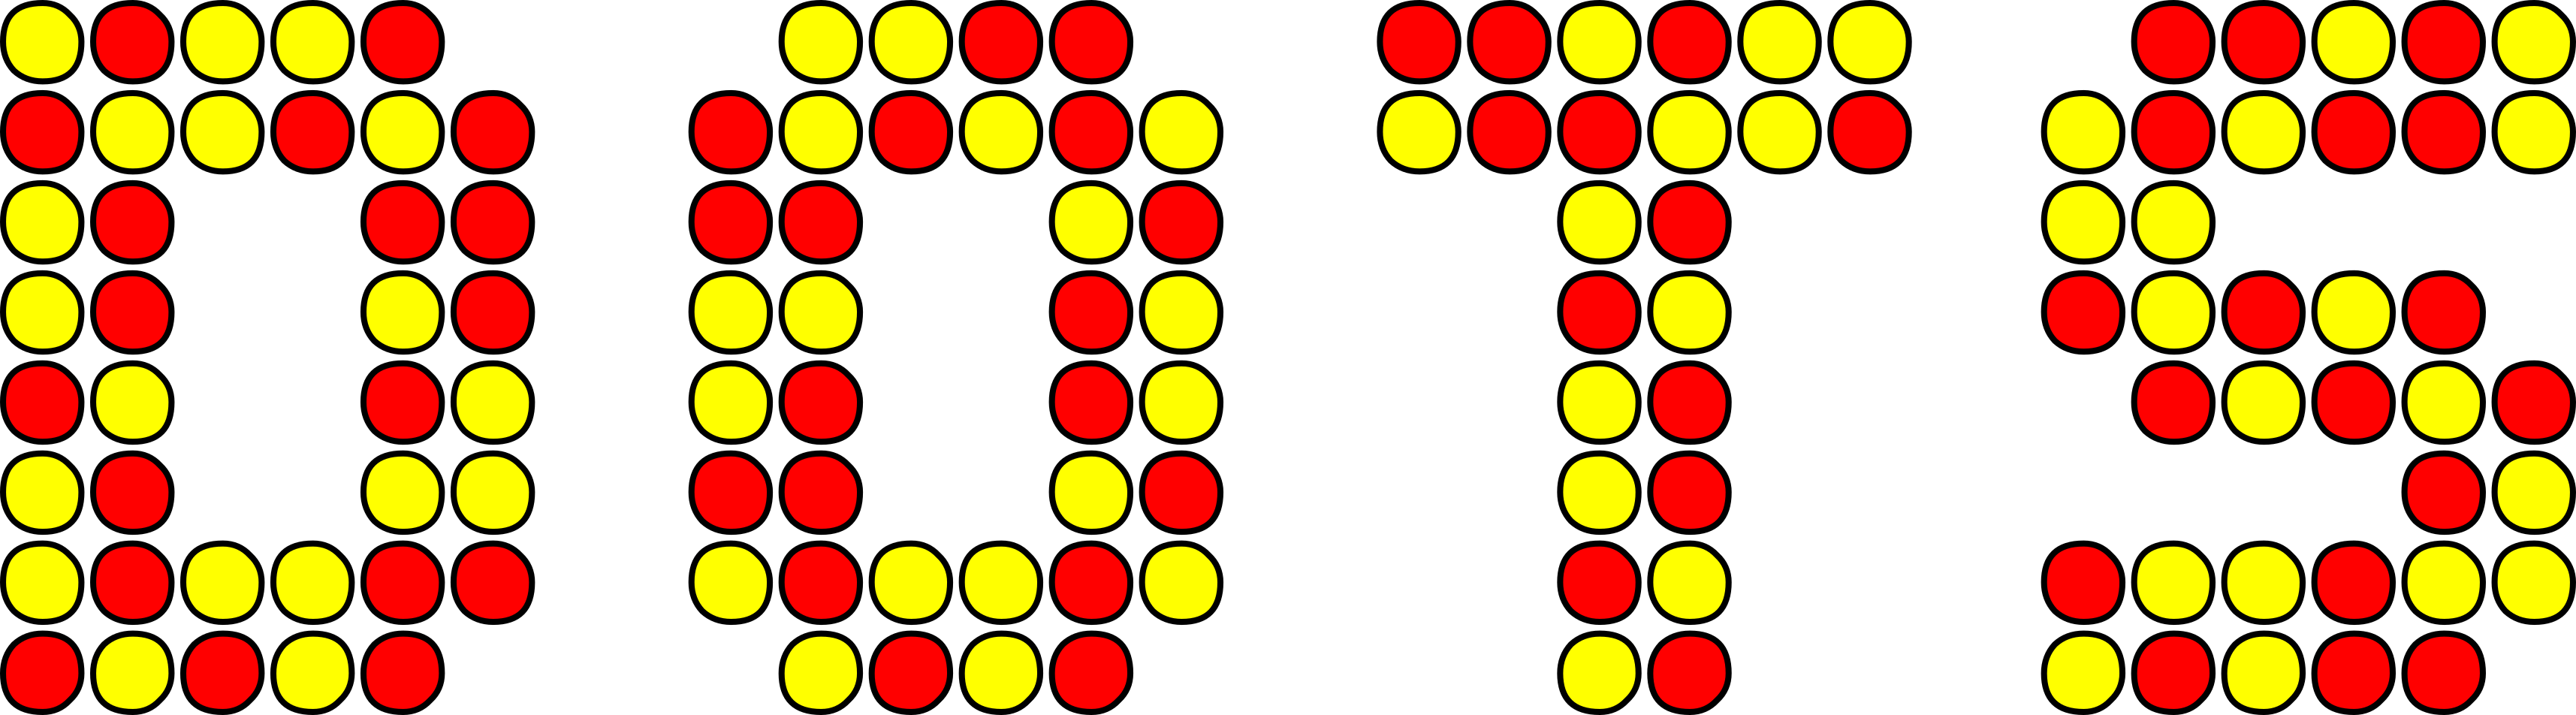
\includegraphics[width=\textwidth]{dots_logo.png}
\vfill{}
\Large
\setmainfont{Tex Gyre Schola}
Designed by Michael Purcell
\end{center}
}%
%\newpage
%\thispagestyle{empty}
%\phantom{a}

\newpage
\setmainfont{Tex Gyre Schola}%
\raggedright%
\section*{Overview}
Permutations is a card game for three or four players.
It is designed for players who are at least eight years old and can be played in
approximately thirty minutes.

\vfill

\section*{Components}
Permutations is played with a deck of forty-eight cards.
There are twelve cards in each of four colours: red, yellow, green, and blue.
Each card displays a unique number between one and forty-eight.

\vfill

\section*{Set Up}
\begin{enumerate}[leftmargin=*]
%	\item Sort the cards by colour.
	\item For a three-player game, remove all the cards of any one colour from the deck.
%	\item Draw a random card of each colour that you are using and place them face up on the table.
%	\item Give each player all of the remaining (eleven) cards of a single colour.
	\item Shuffle the cards.
	\item Deal eleven cards to each player.
	\item Place the remaining cards face up on the table.
	\item Prepare a notepad that you can use to track players' scores throughout the game.
\end{enumerate}

\newpage

\section*{Playing the Game}
The game takes place over a series of \emph{rounds}.

Each round is comprised of eleven \emph{auctions}.
During each auction, you will \emph{draft} one card.
At the end of each round, you will score points based on the cards that you drafted during that round.

You will also use the cards that you draft during each round as your hand for the next round.

The game ends when any player has scored a total of one hundred points or more.
You win if you have the highest score at the end of the game.

\vfill

\subsection*{Auctions}
During an auction, each player will draft one card from a \emph{pool} of available cards.
For the first auction, the pool is comprised of four random cards.
Subsequently, the pool is comprised of the players' bids from the previous auction.

%\newpage

To conduct an auction, secretly choose one card from your hand to be your \emph{bid}.
The value of your bid is the number displayed on your card.
After everyone has chosen, you should reveal your bids.
In decreasing order of bid values, each player should draft one card from the pool.
Place the card that you draft face up in front of you.

\newpage

\subsection*{Scoring}
Your score for each round depends on the cards that you drafted during that round.
To determine your score, first count how many cards you drafted of each colour.
Your score depends only on the largest of these counts, your \emph{max}.
The following table describes your score for each possible max.

\medskip

{
\small
\begin{tabular}{l rrrrrrrrr} \toprule
Max & 3 & 4 & 5 & 6 & 7 & 8 & 9 & 10 & 11 \\ \midrule
Score & 6 & 10 & 15 & 21 & 28 & 36 & 45 & 55 & 66 \\
\bottomrule
\end{tabular}
}

\medskip

These are triangular numbers. If your max for a given round is $m$, then your score is $m(m+1)/2$. 

\vfill

\subsection*{Additional Rounds}
Record the total points each player has scored on a notepad. If no one has scored a total one hundred points or more, you should play another round. You will use the cards that you drafted in the previous round as your hand for the next round.
\vfill
\hrulefill

\textbf{Game Design}: Michael Purcell\\
\textbf{Contact}: \href{mailto:permfair.game@gmail.com}{permfair.game@gmail.com}\\
\begin{tabular}{@{}m{\columnwidth-\widthof{\Huge{\doclicenseIcon}}-0.5cm}@{\hspace{0.05cm}}m{\widthof{\Huge{\doclicenseIcon}}}@{}}
{\textbf{License}: This work is licensed\newline under a ``CC BY 4.0'' license.} & \Huge{\doclicenseIcon}\\
\end{tabular}

%\newpage
%\thispagestyle{empty}
%\phantom{a}
%
%\newpage
%\thispagestyle{empty}
%\phantom{a}
\end{document}
